\documentclass[10pt,twocolumn,letterpaper]{article}

\usepackage[letterpaper,textwidth=6.95in,textheight=9.05in,columnsep=0.28in,top=0.92in]{geometry}
\usepackage{newtxtext,newtxmath}
\usepackage{amsmath}
\usepackage{graphicx}
\usepackage{booktabs}
\usepackage{multirow}
\usepackage{xcolor}
\usepackage{microtype}
\usepackage{hyperref}
\usepackage{caption}
\usepackage{enumitem}
\usepackage{titlesec}
\usepackage{fancyhdr}
\usepackage{flushend}

\titleformat{\section}{\large\bfseries}{\thesection}{0.6em}{}
\titleformat{\subsection}{\normalsize\bfseries}{\thesubsection}{0.55em}{}
\titlespacing*{\section}{0pt}{7pt plus 1.5pt minus 1pt}{2.8pt plus 0.6pt}
\titlespacing*{\subsection}{0pt}{5pt plus 1pt minus 0.8pt}{2pt plus 0.4pt}
\titlespacing*{\paragraph}{0pt}{3.2pt plus 0.5pt minus 0.4pt}{0.55em}

\hypersetup{
  colorlinks=true,
  linkcolor=blue!55!black,
  citecolor=blue!55!black,
  urlcolor=blue!55!black,
  pdftitle={From Pixels to Circuits: Bidirectional 3D Biomechanical Digital Twins and Mechanistic Neural Control Across Species in Annolid},
  pdfauthor={Anonymous Authors}
}

\pagestyle{fancy}
\fancyhf{}
\renewcommand{\headrulewidth}{0pt}
\fancyhead[C]{\small\color{gray!70!black}From Pixels to Circuits \quad$\cdot$\quad Bidirectional 3D Biomechanical Digital Twins \& Neural Control}
\fancyfoot[C]{\small\thepage}
\fancypagestyle{plain}{%
  \fancyhf{}
  \renewcommand{\headrulewidth}{0pt}
  \fancyhead[C]{\small\color{gray!70!black}Preprint \quad$\cdot$\quad November 2026}
  \fancyfoot[C]{\small\thepage}
}

\captionsetup{font=footnotesize,labelfont=bf,skip=3.5pt}
\setlength{\textfloatsep}{7.5pt plus 1.5pt minus 1.5pt}
\setlength{\dbltextfloatsep}{8.5pt plus 1.5pt minus 1.5pt}
\setlength{\floatsep}{6.5pt plus 1.5pt minus 1.5pt}
\setlength{\intextsep}{6.5pt plus 1.5pt minus 1.5pt}
\renewcommand{\topfraction}{0.92}
\renewcommand{\dbltopfraction}{0.92}
\renewcommand{\textfraction}{0.07}

\title{\vspace{-2.0em}\Large\textbf{From Pixels to Circuits: Bidirectional 3D Biomechanical Digital Twins\\and Mechanistic Neural Control Across Species in Annolid}\vspace{-0.4em}}

\author{
  Anonymous Authors
}
\date{\vspace{-1.4em}}

\begin{document}
\raggedbottom
\maketitle
\thispagestyle{plain}

\setlength{\abovedisplayskip}{4.5pt}
\setlength{\belowdisplayskip}{4.5pt}

% =========================================================================
% ABSTRACT
% =========================================================================
\begin{abstract}
\vspace{-0.3em}
A central ambition of computational neuroethology is to move seamlessly from video recordings of freely behaving animals to mechanistic explanations of the bodies and neural circuits that generate those movements. In practice, however, the field remains split across two largely disconnected worlds. Top-down embodied reinforcement-learning platforms produce fluid locomotion in physics engines, yet rely on GPU clusters and black-box policies that lack identified biological cell types. Conversely, bottom-up connectome and spinal-circuit models preserve neurobiological identity, yet remain isolated from multi-view video tracking, anatomical 3D reconstruction, and inverse biomechanics.

Here we introduce a lightweight, bidirectional digital-twin framework inside Annolid that unites video kinematics, physically grounded 3D bodies, and mechanistic neural controllers across three model organisms: \emph{Rattus norvegicus}, \emph{Mus musculus}, and \emph{Drosophila melanogaster}. First, we combine distortion-aware multi-view triangulation, leave-one-out outlier rejection, robust monocular depth lifting, and rigid-skeleton Position-Based Dynamics to reconstruct anatomically faithful 3D trajectories, cutting 4-camera localization error by 45.1\% under severe jitter ($\sigma=6$\,px, Wilcoxon $p=1.6\times 10^{-11}$), shrinking bone-length variability 60-fold, and rejecting 100\% of 65\,px single-view outliers. Second, we pair cross-schema body-scale alignment with bounded 31-degree-of-freedom rodent inverse kinematics and an exact closed-form Karush--Kuhn--Tucker solver for antagonistic spring-muscle forces, auditing the entire pipeline against independent rigid-body rat (0.36\,kg) and mouse (25.6\,g) quadrupeds in MuJoCo~3.5.0. Third, invoking Froude dynamic similarity alongside stride-windowed Hilbert phase analysis, we blindly infer brainstem drive and speed-matched $V0$ and $V3$ spinal interneuron deficits at 100.0\% accuracy (180/180 trials at 4\,mm noise, McNemar $p=1.5\times 10^{-33}$), transferring zero-shot to noisy MuJoCo rats (92--100\%) and to millimeter-scale DANNCE mice experiencing 8\% paw occlusion (92--100\%). Fourth, we equip whole-CNS \emph{Drosophila} spiking connectomes with in-silico optogenetics, Kir2.1 silencing, and dopaminergic Mushroom Body plasticity---including a 2,000-Kenyon-cell sparse olfactory memory that learns ten odors and reverses a single contingency without disrupting the other nine---while demonstrating that 78-neuropil modular connectivity accelerates full 166,700-neuron MaleCNS substeps by 19--23\% (2.95--13.67\,ms) within 200\,MB of CPU memory. Together, these advances bring causal, cross-species neuro-biomechanical modeling directly into routine desktop behavioral workflows.
\end{abstract}

% =========================================================================
% 1. INTRODUCTION
% =========================================================================
\section{Introduction}

Watch a mouse accelerate across a runway or a fruit fly break from walking into grooming, and one immediately confronts the central puzzle of motor neuroscience: how does a nervous system sculpt agile, adaptive behavior through a compliant physical body~\cite{krakauer2017neuroscience,datta2019computational}? Over the past two years, three lines of research have converged to make this question tractable at unprecedented resolution. Deep markerless pose estimators now track dozens of anatomical landmarks across multiple views~\cite{mathis2018deeplabcut,pereira2022sleap,dunn2021dannce,karashchuk2021anipose}, feeding latent behavioral-neural embeddings that dissect movement into sub-second motifs~\cite{weinreb2024keypointmoseq,schneider2023cebra}. In parallel, anatomically calibrated musculoskeletal bodies in MuJoCo~\cite{todorov2012mujoco} and GPU-accelerated MJX---including the Virtual Rodent~\cite{aldarondo2024virtualrodent}, FlyBody~\cite{vaxenburg2025flybody}, NeuroMechFly~v2~\cite{wangchen2024neuromechfly2}, MIMIC-MJX~\cite{zhang2025mimicmjx}, and the 38-degree-of-freedom Rat~v2 model~\cite{bhattasali2026ratncap}---capture ground contact, wing aerodynamics, and antagonistic joint compliance. At the same time, complete electron-microscopy wiring diagrams of the \emph{Drosophila} brain and ventral nerve cord---FlyWire~\cite{dorkenwald2024flywire}, MANC~\cite{takemura2024manc}, and MaleCNS~v1.0 spanning 166,700 neurons~\cite{berg2025malecns}---have catalyzed biophysical Leaky Integrate-and-Fire (LIF) brain simulations~\cite{shiu2024drosophilalif}, while mammalian spinal circuit priors (\emph{Rat NCAP})~\cite{bhattasali2022ncap,bhattasali2026ratncap} explain how speed-dependent gaits and genetic ablation phenotypes~\cite{bellardita2015v0,danner2017spinal} emerge from identified commissural interneurons without imitation learning.

Yet for an experimental neuroethologist working at the bench, a frustrating \emph{two-way integration chasm} still separates these tools. Moving from video to mechanism (\emph{Real-to-Sim}), raw pose estimates stretch and compress rigid bones, lose limbs to single-camera occlusions, and terminate as unstructured 3D point clouds. They yield neither anatomically valid joint trajectories, nor muscle activations, nor quantitative hypotheses about which spinal or descending circuits produced an observed behavioral deficit. Moving in the reverse direction (\emph{Sim-to-Real}), deep reinforcement-learning controllers excel at mimicking kinematics, but their hidden units bear no one-to-one correspondence to genetically defined cell types ($V0_d$, $V0_v$, $V3$, DNp09, MDN, Pair1, or aDN1). Meanwhile, specialist simulators often demand heavy JAX and GPU stacks that sit awkwardly outside everyday annotation software.

\begin{figure*}[t]
  \centering
  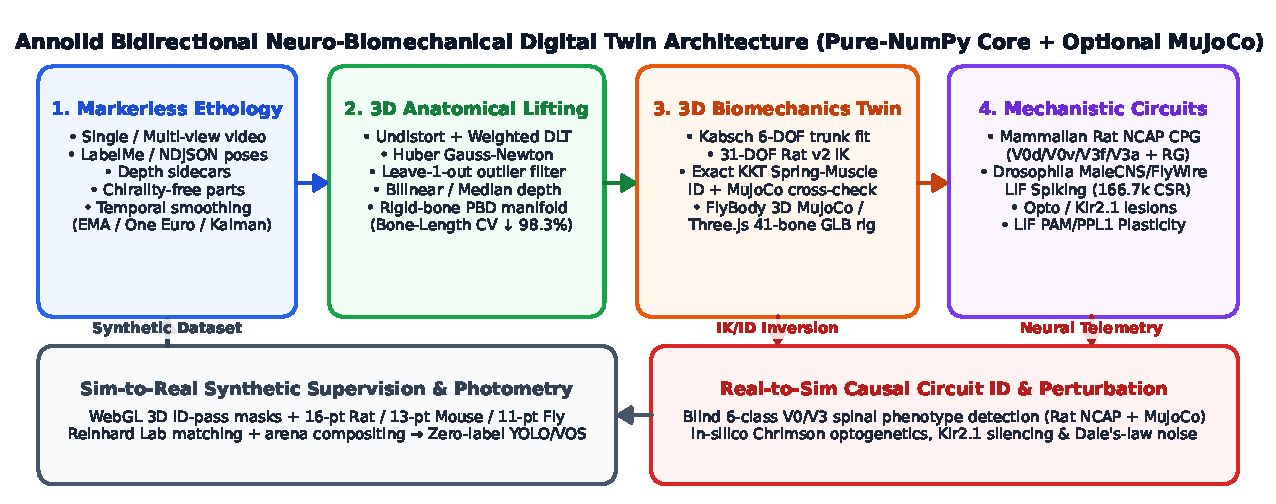
\includegraphics[width=0.98\textwidth]{figures/fig1_architecture.pdf}
  \caption{\textbf{Bidirectional neuro-biomechanical digital twin architecture in Annolid.} (1)~Single- or multi-view video tracking, depth maps, and temporal filters supply raw behavioral measurements. (2)~Distortion-aware multi-view triangulation, leave-one-out outlier rejection, robust depth lifting, and rigid-skeleton Position-Based Dynamics (PBD) recover anatomically consistent 3D trajectories (cutting bone-length variability by 98.3\%). (3)~Cross-schema alignment, Sim(3) body-scale normalization, Kabsch trunk fitting, bounded 31-DOF inverse kinematics, and an exact closed-form KKT antagonistic spring-muscle solver link observed motion to musculoskeletal states, audited against independent MuJoCo~3.5.0 rat and mouse quadrupeds alongside optional FlyBody physics and Three.js rendering. (4)~Mechanistic controllers span mammalian spinal rhythm generation ($V0_d$/$V0_v$/$V3_f$/$V3_a$) scaled by Froude similarity and sparse \emph{Drosophila} whole-CNS LIF connectomes supporting optogenetics, Kir2.1 silencing, and 2,000-Kenyon-cell dopaminergic plasticity.}
  \label{fig:arch}
\end{figure*}

In this work, we close that bidirectional loop directly inside Annolid (Figure~\ref{fig:arch}) using a strictly lean pure-NumPy core that runs faster than real time on an ordinary laptop CPU while interoperating seamlessly with MuJoCo physics and browser-based 3D visualization. Rather than treating tracking, biomechanics, and neural control as separate pipelines, we organize them around four coupled capabilities:

\paragraph{Anatomically faithful 3D lifting from imperfect cameras.}
We pair Brown--Conrady lens undistortion, confidence-weighted Direct Linear Transform (DLT) initialization, leave-one-out outlier pruning, and Huber Gauss--Newton refinement with monocular depth lifting and \emph{rigid-skeleton} Position-Based Dynamics (PBD). Explicitly separating rigid axial bones from articulated limb chords resolves a subtle failure mode in standard skeleton smoothing and exposes a clean bias--variance tradeoff between spatial-only and temporally regularized projection across Gaussian jitter, extreme single-view outliers, and heavy camera dropout.

\paragraph{Cross-species inverse kinematics, exact muscle-force inversion, and an independent physics audit.}
We introduce automatic ingestion of widely used rodent landmark conventions (including DANNCE/Rat7M, Anipose, LocoMouse, and SLEAP), isotropic Sim(3) unit and body-scale detection, Kabsch 6-DOF trunk alignment, anatomically bounded 31-DOF inverse kinematics, and a closed-form Karush--Kuhn--Tucker (KKT) solver for antagonistic spring-muscle activations. To avoid the circularity of testing an inverse solver only on data from its own generative model, we audit our pipeline against two independent rigid-body quadrupeds built in MuJoCo~3.5.0---a 0.36\,kg rat and a 25.6\,g mouse---establishing both where kinematic transfer excels and where decoupled surrogate torques diverge from full contact-coupled Lagrangian mechanics.

\paragraph{Cross-species blind inference of hidden spinal circuit states.}
By diagnosing three statistical artifacts that corrupt noisy gait analysis---Rayleigh velocity inflation, broadband phase noise, and a tight walk-versus-trot symmetry boundary---and invoking Alexander \& Jayes' Froude dynamic similarity~\cite{alexander1983froude}, we construct a noise-robust estimator that blindly infers brainstem drive and distinguishes speed-matched $V0$ and $V3$ commissural interneuron deficits directly from 3D tracks, generalizing zero-shot across both physics engines and mammalian body sizes even under intermittent paw occlusion.

\paragraph{Causal perturbations, sparse olfactory memory, and modular whole-CNS scaling in \emph{Drosophila}.}
Finally, we extend sparse Compressed Sparse Row (CSR) whole-CNS connectomes with timed Chrimson optogenetics, Kir2.1 silencing, Dale's-law synaptic noise, and three-factor dopaminergic Mushroom Body plasticity scaling up to a 2,000-Kenyon-cell (KC) sparse associative memory. We verify closed-loop motor outputs across five natural behaviors, prove that multi-neuron population redundancy confers noise resilience over single-unit rate approximations, and benchmark complete 166,700-neuron MaleCNS~v1.0 spiking substeps on biologically clustered 78-neuropil graphs against random Erd\H{o}s--R\'enyi baselines.

% =========================================================================
% 2. RELATED WORK
% =========================================================================
\section{The Emerging Landscape of Embodied Neuroethology}

The past two years have witnessed rapid convergence across behavioral tracking, musculoskeletal simulation, and circuit-constrained control (Table~\ref{tab:landscape}). Three complementary traditions frame our contribution.

\begin{table*}[t]
\centering
\caption{\textbf{Synthesis of recent frameworks spanning digital animal behavior, 3D biomechanics, and neural control.} Annolid unites markerless 3D lifting, bounded inverse kinematics and muscle-force inversion, cell-type-specific causal perturbations, and Sim-to-Real supervision in a pure-NumPy desktop core with optional MuJoCo interoperability.}
\label{tab:landscape}
\scriptsize
\setlength{\tabcolsep}{3.4pt}
\resizebox{\textwidth}{!}{%
\begin{tabular}{@{}lcccccc@{}}
\toprule
\textbf{Framework / Study} & \textbf{Benchmarked Species} & \textbf{Neural Control Paradigm} & \textbf{3D Lifting / IK} & \textbf{Muscle ID} & \textbf{Cell-Type Causal} & \textbf{Core Runtime} \\
\midrule
Anipose~\cite{karashchuk2021anipose} / DANNCE~\cite{dunn2021dannce} & Multi / Rodent & None (Tracking) & Multi-view / 3D CNN & No & No & Python / PyTorch \\
Virtual Rodent~\cite{aldarondo2024virtualrodent} & Rat & Black-box Deep RL & External MoCap & No & No & MuJoCo + GPU RL \\
MIMIC-MJX / STAC-MJX~\cite{zhang2025mimicmjx} & Rat / Mouse / Fly & Imitation Deep RL & GPU MJX IK & No & No & JAX + MuJoCo-MJX \\
FlyBody~\cite{vaxenburg2025flybody} & \emph{Drosophila} & Deep RL (Walk/Flight) & Optional IK & No & No & MuJoCo + dm\_control \\
NeuroMechFly~v2~\cite{wangchen2024neuromechfly2} & \emph{Drosophila} & Hierarchical CPG + Vision & Replay / Sim & No & Partial (CPG) & MuJoCo (FlyGym) \\
FlyWire LIF~\cite{shiu2024drosophilalif} & \emph{Drosophila} & Whole-Brain Spiking LIF & Disembodied & No & Yes (Opto/Lesion) & Brian2 / PyTorch \\
Rat NCAP~\cite{bhattasali2026ratncap} & Rat (Rat~v2) & Spinal CPG Priors (RL) & Forward Sim & Spring-Muscle & Yes ($V0$/$V3$ Ablation) & MuJoCo / MJX + JAX \\
\midrule
\textbf{Annolid Digital Twin (Ours)} & \textbf{Rat + Mouse + Fly} & \textbf{MaleCNS LIF + Rat NCAP} & \textbf{Multi-View + Depth + IK} & \textbf{Exact KKT ID} & \textbf{Opto + Kir2.1 + $V0$/$V3$} & \textbf{Pure NumPy (+Opt.\ MJ)} \\
\bottomrule
\end{tabular}}
\end{table*}

\paragraph{Top-down embodied reinforcement learning.}
A major breakthrough of the virtual-animal paradigm is the demonstration that artificial policies trained to imitate physical behavior spontaneously organize internal representations resembling biological motor circuits. Aldarondo et~al.~\cite{aldarondo2024virtualrodent} showed that latent states of a MuJoCo virtual rat predict motor cortical and striatal population dynamics better than kinematics alone because the policy must solve inverse dynamics under gravity and contact. Vaxenburg et~al.~\cite{vaxenburg2025flybody} extended this approach to \emph{FlyBody}, an anatomically rich fruit fly capable of walking and vision-guided flight, while Zhang et~al.~\cite{zhang2025mimicmjx} scaled imitation learning across rodents, flies, stick insects, and nematodes via GPU-parallel \emph{MIMIC-MJX}. Despite their expressive power, end-to-end policies remain opaque to genetic perturbation: one cannot silence $V0_d$ commissural interneurons or activate Moonwalker descending neurons inside a standard multilayer perceptron, and training requires substantial GPU infrastructure.

\paragraph{Bottom-up mechanistic and connectome-constrained control.}
Working from anatomy upward, whole-CNS electron microscopy of \emph{Drosophila}---spanning the 139,000-neuron FlyWire female brain~\cite{dorkenwald2024flywire}, the 23,000-neuron MANC ventral nerve cord~\cite{takemura2024manc}, and the 166,700-neuron MaleCNS~v1.0 wiring diagram~\cite{berg2025malecns}---has enabled whole-brain spiking models that predict behavioral responses to targeted optogenetic perturbations~\cite{shiu2024drosophilalif}, complemented by biomechanical testbeds such as NeuroMechFly~v2~\cite{wangchen2024neuromechfly2}. In mammals, biophysical network models by Danner et~al.~\cite{danner2017spinal} explained how speed-recruited commissural ($V0_d$, $V0_v$, $V3$) and long propriospinal pathways orchestrate gait transitions and account for Bellardita \& Kiehn's~\cite{bellardita2015v0} discovery that $V0$ ablation forces trotting mice into premature bounding. Recently, Bhattasali et~al.~\cite{bhattasali2026ratncap} embedded these spinal architectural priors (\emph{Rat NCAP}) inside a 38-DOF Rat~v2 body driven by antagonistic spring muscles, achieving emergent walk--trot--bound transitions without imitation targets.

\paragraph{3D pose reconstruction and behavioral quantification.}
On the experimental side, calibrated triangulation suites such as Anipose~\cite{karashchuk2021anipose} and volumetric networks such as DANNCE~\cite{dunn2021dannce} recover 3D markerless keypoints, while Keypoint-MoSeq~\cite{weinreb2024keypointmoseq} and CEBRA~\cite{schneider2023cebra} uncover behavioral syllables and joint neural-behavioral manifolds. Still, most ethology workflows stop at Cartesian trajectories, leaving a gulf between pose estimation and mechanistic circuit testing. Annolid bridges all three layers in one accessible, desktop-ready environment.

% =========================================================================
% 3. ARCHITECTURE & MATHEMATICAL FORMULATION
% =========================================================================
\section{Architecture and Mathematical Formulation}

\subsection{From Noisy Multi-View Cameras to Anatomically Consistent 3D Motion}

\paragraph{Calibrated triangulation and consensus outlier pruning.}
In a multi-camera arena with $M$ synchronized views, each camera $c \in \{1,\dots,M\}$ is characterized by intrinsics $\mathbf{K}_c = (f_x, f_y, c_x, c_y)$, world-to-camera extrinsics $(\mathbf{R}_c, \mathbf{t}_c)$, and Brown--Conrady lens distortion $\mathbf{d}_c = (k_1, k_2, p_1, p_2, k_3)$. Because lens distortion warps peripheral keypoints across wide-angle behavioral cages, raw 2D detections $\mathbf{u}_c = (u_c, v_c)$ with confidence $s_c$ are first undistorted by fixed-point inversion of the radial-tangential distortion map. Whenever a landmark appears in $M \ge 2$ views, we form an initial 3D estimate $\mathbf{X}_0 \in \mathbb{R}^3$ via confidence-weighted Direct Linear Transform (DLT) singular value decomposition on the rows $\sqrt{s_c}(u_c \mathbf{p}_{c,3}^\top - \mathbf{p}_{c,1}^\top)$ and $\sqrt{s_c}(v_c \mathbf{p}_{c,3}^\top - \mathbf{p}_{c,2}^\top)$ of the projection matrix $\mathbf{P}_c = \mathbf{K}_c[\mathbf{R}_c \mid \mathbf{t}_c]$, and refine $\mathbf{X}$ with damped Gauss--Newton iterations under a Huber robust loss ($\delta = 4$\,px):
\begin{equation}
  \min_{\mathbf{X}\in\mathbb{R}^3} \sum_{c \in \mathcal{V}} s_c \, \rho_\delta\!\left(\left\|\pi_c(\mathbf{X}) - \mathbf{u}_c\right\|_2\right).
\end{equation}

Real pose detectors occasionally suffer catastrophic single-view identity swaps or reflection glitches that pull ordinary least-squares triangulation centimeters off target. When $|\mathcal{V}| \ge 3$ and the worst reprojection residual exceeds a threshold $\tau_{\mathrm{out}}$, greedy leave-one-out consensus pruning removes whichever single view yields the largest reduction in worst-case reprojection error before final refinement. For single-camera setups paired with depth sensors or monocular depth estimators, our depth lifter supports both subpixel bilinear interpolation (for smooth depth maps) and spike-resistant $(2r+1)\times(2r+1)$ median-patch sampling (for noisy depth boundaries), transforming lifted camera coordinates into world space via $\mathbf{X}_w = \mathbf{R}_c^\top(\mathbf{X}_c - \mathbf{t}_c)$.

\paragraph{Rigid-skeleton Position-Based Dynamics.}
Even after robust triangulation, independent frame-by-frame estimates violate skeletal geometry: cranial and vertebral segments expand and contract from frame to frame. A tempting remedy is to constrain every edge of a visualization skeleton to a constant length. However, that approach carries an anatomical trap: chord distances linking the thorax or pelvis directly to a paw naturally shorten and lengthen by tens of millimeters across stance and swing. Constraining those articulated chords injects systematic bias even into noiseless recordings.

We therefore restrict geometric projection strictly to the set of \emph{rigid} anatomical segments $\mathcal{E}_{\mathrm{rigid}}$---the 11 cranial, axial, and caudal bones of the rodent skeleton---while leaving articulated limb chords unconstrained. Canonical segment lengths $L_{ij}$ are learned automatically from the confidence-weighted temporal median across the recording. Each frame is then projected onto the rigid-bone manifold via confidence-weighted Position-Based Dynamics (PBD), paired with optional Laplacian temporal acceleration smoothing ($\lambda_t \in [0, 0.15]$):
\begin{align}
  \Delta \mathbf{x}_i &= +\frac{w_i^{-1}}{w_i^{-1} + w_j^{-1}}\, \alpha \left(\|\mathbf{x}_j - \mathbf{x}_i\| - L_{ij}\right)\hat{\mathbf{u}}_{ij}, \\
  \Delta \mathbf{x}_j &= -\frac{w_j^{-1}}{w_i^{-1} + w_j^{-1}}\, \alpha \left(\|\mathbf{x}_j - \mathbf{x}_i\| - L_{ij}\right)\hat{\mathbf{u}}_{ij},
\end{align}
where inverse-mass weights $w_i = \max(s_i, 0.05)^p$ anchor high-confidence detections while drawing uncertain or partially occluded endpoints smoothly back onto the bone manifold. Separating spatial projection ($\lambda_t = 0$) from temporal damping ($\lambda_t = 0.15$) lets experimentalists preserve sharp kinematics in sub-pixel calibrated rigs while suppressing severe triangulation noise in noisier recordings.

\subsection{Cross-Species Body Alignment, Inverse Kinematics, and Antagonistic Muscle Forces}

\paragraph{Cross-schema normalization and Kabsch trunk alignment.}
Behavioral laboratories rarely share identical keypoint names, length units, or animal sizes: volumetric DANNCE and Rat7M exports report millimeter landmarks such as anterior head, spine segments, and hand/foot sites, whereas Anipose, LocoMouse, SLEAP, and MuJoCo use distinct labels in meters or centimeters. To eliminate tedious manual preprocessing, our ingestion stage maps case-insensitive aliases across these common conventions onto canonical rodent anatomy, bridges brief tracking dropouts by linear interpolation across missing frames, and inspects the temporal median of pairwise cranial and trunk distances relative to canonical Rat~v2 proportions ($d_{\mathrm{obs}} / d_{\mathrm{ref}}$). This automatically identifies both measurement units (millimeters if $>15\times$ canonical, centimeters if $>2.5\times$, else meters) and isotropic Sim(3) body scale $s$. Scales near unity ($s \in [0.80, 1.25]$) snap to $1.0$ to preserve canonical rat calibration, whereas a 25\,g laboratory mouse is automatically detected at $s \approx 0.35$.

To construct an egocentric body frame without leaking limb motion into trunk pose, we align the seven rigid anterior and cranial landmarks (torso center, thorax, neck, head, nose, and both ears) onto canonical local coordinates $\mathbf{L}_k$ via Kabsch singular value decomposition ($\mathbf{H} = \sum_k \bar{\mathbf{L}}_k \bar{\mathbf{W}}_k^\top = \mathbf{U}\boldsymbol{\Sigma}\mathbf{V}^\top$, $\mathbf{R} = \mathbf{V}\mathrm{diag}(1,1,\det(\mathbf{V}\mathbf{U}^\top))\mathbf{U}^\top$). Estimating root translation from the full seven-landmark centroid $\mathbf{r} = \bar{\mathbf{W}} - \mathbf{R}\bar{\mathbf{L}}$ rather than a single torso marker attenuates root-position jitter by $\sqrt{7} \approx 2.65\times$, preventing common-mode noise from masquerading as synchronous paw motion. Transforming posterior trunk and paw coordinates into body-local space $\mathbf{p}_{\mathrm{loc}} = \mathbf{R}^\top(\mathbf{p}_w - \mathbf{r})$, we recover lumbar bending and all four limb joint chains (8~DOFs per forelimb, 6~DOFs per hindlimb; 31 locomotion DOFs in total) from sagittal excursion $\Delta x$, lateral abduction $\Delta y$, and paw elevation above a robust sequence ground plane ($z_{\mathrm{ground}} = P_{15}(z_{\mathrm{paws}}) - 4$\,mm), strictly clamped within physiological Rat~v2 joint limits.

\paragraph{Exact closed-form muscle-force inversion.}
In Rat NCAP~\cite{bhattasali2026ratncap}, every joint $j \in \{1,\dots,31\}$ is actuated by an antagonistic flexor--extensor pair of linear spring muscles whose reparameterized stiffnesses $(k_{f,j}, k_{e,j})$ and offsets $(c_{f,j}, c_{e,j})$ match exact equilibrium at co-activation $a_f = a_e = 1, q = q_{\mathrm{eq}}$:
\begin{align}
  \tau_j &= a_{e,j} A_j(q_j) - a_{f,j} B_j(q_j) - k_{d,j} \dot{q}_j, \\
  A_j(q_j) &= k_{e,j}(q^{\mathrm{hi}}_j - q_j + c_{e,j}) \ge 0, \nonumber\\
  B_j(q_j) &= k_{f,j}(q_j - q^{\mathrm{lo}}_j + c_{f,j}) \ge 0. \nonumber
\end{align}
Recovering two muscle activations $(a_{f,j}, a_{e,j}) \in [0,1]^2$ from a single required surrogate torque $\tau_{\mathrm{req},j} = I_j \ddot{q}_j + d_j \dot{q}_j$ is mathematically underdetermined because opposing muscles can co-contract without altering net torque. Rather than running slow iterative optimization at every frame, we formulate the strictly convex minimum-deviation problem around physiological baseline tone $c_0 = 0.45$:
\begin{equation}
  \min_{a_e, a_f \in [0,1]} \tfrac{1}{2}\!\big[(a_e - c_0)^2 + (a_f - c_0)^2\big]
  \;\;\text{s.t.}\;\; A a_e - B a_f = y,
\end{equation}
with $y = \tau_{\mathrm{req}} + k_d \dot{q}$. Because the objective is quadratic with one linear equality constraint, its unique global optimum admits an $O(1)$ closed-form KKT solution:
\begin{equation}
  \lambda^\star = \frac{y - (A - B)c_0}{A^2 + B^2}, \;\; a_e^\star = c_0 + \lambda^\star A, \;\; a_f^\star = c_0 - \lambda^\star B,
\end{equation}
followed by exact active-set projection onto $[0,1]^2$ whenever a muscle saturates. This reproduces feasible surrogate torques to machine precision ($0.0000$\,Nm residual) while reporting positive and negative mechanical power $P^\pm = \sum_j (\tau_j \dot{q}_j)^\pm$, effective joint stiffness $k_{\mathrm{eff},j} = a_{e,j} k_{e,j} + a_{f,j} k_{f,j}$, and Cost of Transport $\mathrm{CoT} = \overline{|P|} / (mg\bar{v})$.

\subsection{Inferring Hidden Spinal Circuit States from Freely Moving Kinematics}

A central goal of behavioral phenotyping is to infer hidden neural circuit alterations non-invasively from gait videos. Doing so reliably in the presence of realistic 3D tracking jitter requires overcoming three distinct failure modes that quietly break naive kinematic classifiers:

\begin{enumerate}[leftmargin=*,itemsep=1.4pt,topsep=2pt]
  \item \textbf{Rayleigh velocity inflation.} Naive frame-to-frame speed $\|\mathbf{r}_{t+1}-\mathbf{r}_t\|/\Delta t$ rectifies isotropic tracking noise into a strictly positive speed bias of $\frac{\sqrt{\pi}}{2}\frac{\sqrt{2}\sigma_r}{\Delta t} \approx 0.13$\,m/s at $\sigma_{\mathrm{3D}}=4$\,mm, turning stationary animals into apparent walkers. Computing median displacement velocity over a stride-scale window $W = \lfloor 0.20/\Delta t \rfloor$ reduces phantom speed tenfold without biasing steady progression.
  \item \textbf{Broadband phase noise and high-frequency mouse cadences.} Under 3D jitter, vertical paw clearance ($\sim$15--24\,mm in rats; $\sim$5--8\,mm in mice) carries more than an order of magnitude higher signal-to-noise ratio than noisy horizontal hip excursion. After interpolating occluded frames, we identify dominant step frequency across $f_{\mathrm{step}} \in [0.8, \min(14.0, 0.48/\Delta t)]$\,Hz---spanning both 1.7--5.5\,Hz rats and 2.5--12\,Hz mice~\cite{bellardita2015v0}---extract amplitude-weighted circular interlimb phase offsets $(\phi_{\mathrm{FL}}, \phi_{\mathrm{HL}}, \phi_{\mathrm{HR}})$ relative to the front-right paw via bandpass Hilbert analysis around $[0.55 f_{\mathrm{step}}, 1.65 f_{\mathrm{step}}]$, and estimate stance duty factor $\beta$ using an edge-preserving three-tap rolling median.
  \item \textbf{The walk-versus-trot symmetry boundary.} Tracking jitter depresses apparent duty factor $\beta$ below $0.72$, forcing classification to rely on diagonal-couplet synchrony $d_{\mathrm{diag}} = \tfrac{1}{2}[d_\circ(\phi_{\mathrm{HL}}, 0) + d_\circ(\phi_{\mathrm{HR}}, \phi_{\mathrm{FL}})]$. Because an ideal four-beat lateral-sequence walk has $d_{\mathrm{diag}} = 0.25$, a loose cutoff ($d_{\mathrm{diag}} < 0.24$) leaves virtually zero noise margin and collapses walks into trots. Setting the decision boundary at the principled Hildebrand midpoint $d_{\mathrm{diag}} < 0.18$ cleanly separates diagonal trots ($0.00\text{--}0.12$) from four-beat walks ($0.23\text{--}0.25$) even under substantial vertical noise.
\end{enumerate}

A further obstacle arises when transferring a rat spinal classifier to mice: a 25\,g mouse trots and bounds at markedly lower absolute speeds than a 360\,g rat. Rather than re-tuning species-specific speed cutoffs, we appeal to Alexander \& Jayes' classic \emph{Froude dynamic similarity hypothesis}~\cite{alexander1983froude}, which predicts that geometrically similar quadrupeds transition between gaits at matched dimensionless Froude numbers $\mathrm{Fr} = v^2 / (gL)$. Using the automatically inferred body scale $s = L / L_{\mathrm{rat}}$, we map physical speed $\bar{v}$ to canonical Froude-equivalent speed $\tilde{v} = \bar{v} / \sqrt{s}$. Combining $\tilde{v}$ with left--right synchrony $S_{\mathrm{LR}} = 1 - 2\min(0.5, \tfrac{1}{2}[d_\circ(\phi_{\mathrm{FL}}, 0) + d_\circ(\phi_{\mathrm{HL}}, \phi_{\mathrm{HR}})])$ yields inferred brainstem drive $\hat{c} = \mathrm{clip}(\tilde{v}, 0, 1)$ and two mechanistic commissural integrity indices grounded in Bellardita \& Kiehn~\cite{bellardita2015v0} and Danner et~al.~\cite{danner2017spinal}:
\begin{align}
  I_{V0} &= \begin{cases} 1 - S_{\mathrm{LR}} & \text{if } \tilde{v} \in [0.16, 0.66]\text{\,m/s}, \\ 1 & \text{otherwise}, \end{cases} \\
  I_{V3} &= \begin{cases} S_{\mathrm{LR}} & \text{if } \tilde{v} > 0.66\text{\,m/s}, \\ 1 & \text{otherwise}. \end{cases}
\end{align}
Premature left--right synchrony inside the moderate trot regime ($I_{V0} \to 0$) diagnoses a $V0$ commissural deficit, whereas persistent alternation at high galloping speeds ($I_{V3} \to 0$, $\tilde{v} \ge 0.72$\,m/s) diagnoses a $V3$ synchrony deficit.

\subsection{Connectome-Constrained Spiking Control, Causal Perturbations, and Olfactory Memory}

To bring the same bidirectional workflow to invertebrate neuroethology, Annolid compiles \emph{Drosophila} Brain+VNC wiring diagrams---ranging from compact 55-population canonical circuits (79 pathways) and individual-neuron spiking expansions (1,470 neurons, 15,860 synapses; 1,534 neurons and 16,340 synapses with associative plasticity) to external MaleCNS~v1.0, FlyWire, and MANC connectivity tables---into $O(|E|)$ Compressed Sparse Row (CSR) synaptic operators. Synaptic weights respect \emph{Drosophila} neurotransmitter polarity (acetylcholine $+1$, GABA $-1$, central glutamate-gated chloride channels $-0.6$, neuromuscular glutamate $+1$, octopamine $+0.85$, dopamine $+0.5$, and serotonin $-0.3$). In spiking mode, each neuron integrates biophysical Leaky Integrate-and-Fire dynamics ($V_{\mathrm{rest}}=-52$\,mV, $V_{\mathrm{th}}=-45$\,mV, refractory period $\tau_{\mathrm{ref}}=2.2$\,ms, synaptic decay $\tau_{\mathrm{syn}}=5$\,ms, substep $\Delta t_{\mathrm{sub}}=0.2$\,ms) with event-driven sparse spike propagation.

Four experimental neuroscience interventions operate natively on these networks: timed Chrimson optogenetic depolarization of any chosen cell class; graded Kir2.1 hyperpolarizing silencing ($k \in [0,1]$ across both rate and spiking substeps); Dale's-law sign-preserving multiplicative synaptic variability ($\max(0.05, 1+\sigma\epsilon)$); and three-factor dopaminergic Mushroom Body plasticity. Beyond a canonical two-odor reversal circuit, we implement a high-dimensional sparse olfactory memory modeled directly on \emph{Drosophila} Mushroom Body anatomy: 50 antennal-lobe Projection Neurons (PNs) project randomly onto $N_{\mathrm{KC}} = 2{,}000$ Kenyon cells with 6 input claws per KC, an Anterior Paired Lateral (APL) global GABAergic interneuron enforces exact 5\% winner-take-all sparsity ($100$ active KCs per odor), and per-KC eligibility traces ($\tau_e = 90$\,ms) drive 4,000 online plastic synapses onto approach and avoidance output neurons (MBONs) under opposing PAM (reward) and PPL1 (punishment) dopaminergic reinforcement: $\Delta w_{k,\mathrm{app}} = \eta e_k (\mathrm{PAM}-\mathrm{PPL1})\Delta t$, $\Delta w_{k,\mathrm{avd}} = -\Delta w_{k,\mathrm{app}}$, bounded in $[0.15, 2.50]$.

% =========================================================================
% 4. RESULTS
% =========================================================================
\section{Results}

All quantitative evaluations execute deterministically on a standard CPU directly against Annolid's production simulation modules. Uncertainty is reported as 2,000-resample bootstrap 95\% confidence intervals (CIs), and paired comparisons are assessed using two-sided Wilcoxon signed-rank, Mann--Whitney~$U$, and exact McNemar tests.

\subsection{Rigid-Skeleton Projection Suppresses Tracking Noise, Outliers, and View Dropouts}

We first evaluated multi-view reconstruction across calibrated 2-, 3-, and 4-camera arenas with realistic Brown--Conrady lens distortion over 60 trotting frames (960 reconstructed 3D landmarks per condition), sweeping 2D Gaussian detector jitter ($\sigma \in [0, 8]$\,px), 20\% single-view 65\,px outlier glitches, 30\% random camera-dropout occlusions, and monocular depth lifting with and without depth-sensor spikes (Figure~\ref{fig:exp1} and Table~\ref{tab:exp1}).

\begin{figure*}[t]
  \centering
  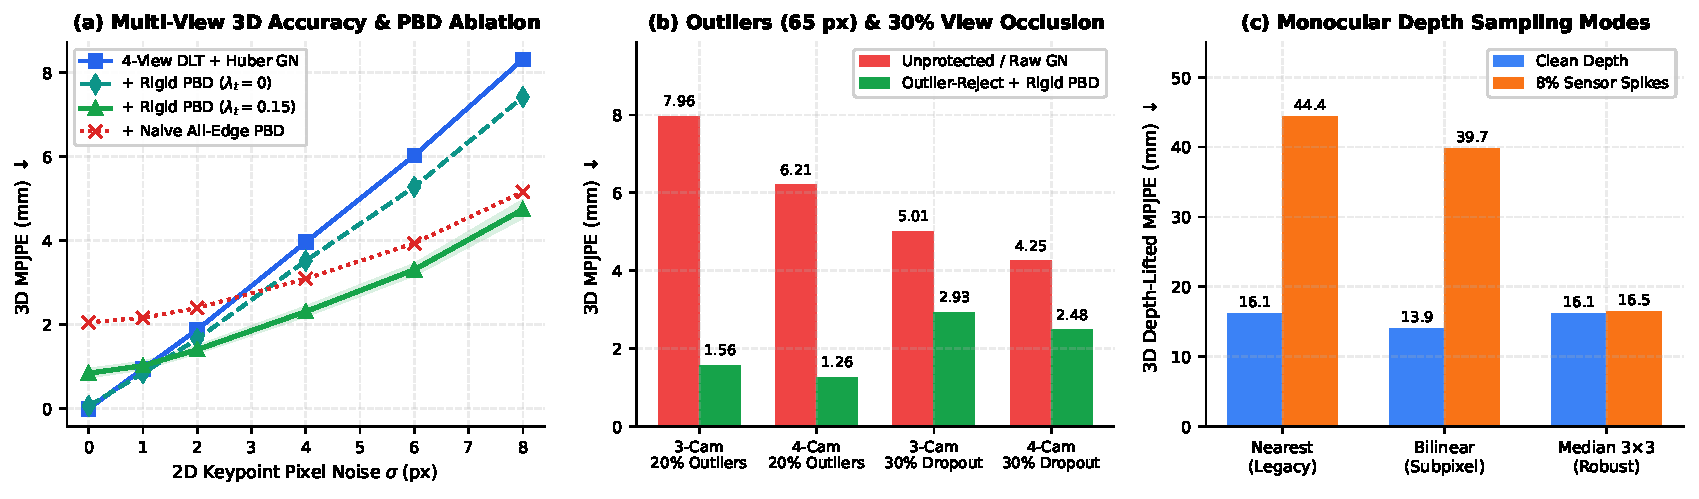
\includegraphics[width=0.98\textwidth]{figures/fig2_multiview_3d_lifting.pdf}
  \caption{\textbf{Multi-view 3D reconstruction, rigid-skeleton ablation, occlusion stress tests, and monocular depth lifting.} (a)~4-camera 3D localization error across 2D detector noise (shaded 95\% bootstrap CIs): spatial-only rigid PBD ($\lambda_t=0$) preserves sub-millimeter precision at $\sigma \le 1$\,px (0.063 and 0.847\,mm vs.\ 0.946\,mm raw Gauss--Newton), whereas adding temporal smoothing ($\lambda_t=0.15$) reduces error by 45.1\% at $\sigma=6$\,px (6.03 $\to$ 3.31\,mm, $p=1.6\times 10^{-11}$). Naive all-edge PBD locks articulated limb chords and introduces a 2.06\,mm bias even with noiseless detections. (b)~Leave-one-out consensus pruning rejects 100.0\% of 65\,px single-view outliers (374/374), and rigid PBD cuts 30\% camera-dropout error by 41.6\% ($p \le 1.7\times 10^{-11}$). (c)~Monocular depth lifting: bilinear interpolation lowers clean error by 13.4\% ($p=1.9\times 10^{-9}$), while $3\times 3$ median-patch filtering cuts 8\%-spike error by 63.0\% ($p=4.4\times 10^{-5}$).}
  \label{fig:exp1}
\end{figure*}

\begin{table}[t]
\centering
\caption{\textbf{Multi-view triangulation, PBD ablation, outlier stress, and 30\% view dropout (60 frames, 960 keypoints).} Mean 3D MPJPE (mm) with 95\% bootstrap CIs and paired Wilcoxon $p$-values comparing temporally regularized rigid-skeleton PBD against DLT+GN.}
\label{tab:exp1}
\scriptsize
\setlength{\tabcolsep}{2.3pt}
\resizebox{\columnwidth}{!}{%
\begin{tabular}{@{}lrrrrrr@{}}
\toprule
\textbf{Setting} & \textbf{DLT+GN} & \textbf{Rigid} & \textbf{Rigid} & \textbf{All-Edge} & \textbf{Bone CV (\%)} & \textbf{Wilcoxon} \\
 & (mm) & ($\lambda_t=0$) & ($\lambda_t=0.15$) [95\% CI] & (mm) & Before $\to$ After & $p$-value \\
\midrule
4-Cam, $\sigma=0$\,px & \textbf{0.00} & 0.06 & 0.85 [0.75, 0.94] & 2.06 & 0.18 $\to$ 0.02 & $1.6\mathrm{e}{-11}$ \\
4-Cam, $\sigma=1$\,px & 0.95 & \textbf{0.85} & 1.02 [0.95, 1.11] & 2.16 & 2.23 $\to$ 0.04 & $7.4\mathrm{e}{-2}$ \\
4-Cam, $\sigma=2$\,px & 1.88 & 1.66 & \textbf{1.41} [1.33, 1.48] & 2.40 & 4.60 $\to$ 0.08 & $8.8\mathrm{e}{-11}$ \\
3-Cam, $\sigma=4$\,px & 4.61 & 4.11 & \textbf{2.66} [2.57, 2.75] & 3.35 & 10.18 $\to$ 0.21 & $1.6\mathrm{e}{-11}$ \\
2-Cam, $\sigma=4$\,px & 6.18 & 5.35 & \textbf{3.44} [3.30, 3.59] & 3.98 & 15.50 $\to$ 0.26 & $1.6\mathrm{e}{-11}$ \\
4-Cam, $\sigma=6$\,px & 6.03 & 5.28 & \textbf{3.31} [3.18, 3.44] & 3.94 & 13.91 $\to$ 0.23 & $1.6\mathrm{e}{-11}$ \\
4-Cam, $\sigma=8$\,px & 8.32 & 7.42 & \textbf{4.74} [4.55, 4.96] & 5.16 & 17.56 $\to$ 0.34 & $1.6\mathrm{e}{-11}$ \\
\midrule
3-Cam + 20\% 65px Out.$^\dagger$ & 7.96$^\ddagger$ & --- & \textbf{1.56} [1.42, 1.74] & --- & 8.81 $\to$ 0.23 & $1.8\mathrm{e}{-11}$ \\
4-Cam + 20\% 65px Out.$^\dagger$ & 6.21$^\ddagger$ & --- & \textbf{1.26} [1.19, 1.33] & --- & 3.70 $\to$ 0.07 & $1.6\mathrm{e}{-11}$ \\
3-Cam + 30\% Dropout & 5.01 & --- & \textbf{2.93} [2.81, 3.05] & --- & 11.28 $\to$ 0.26 & $1.7\mathrm{e}{-11}$ \\
4-Cam + 30\% Dropout & 4.25 & --- & \textbf{2.48} [2.38, 2.59] & --- & 9.86 $\to$ 0.21 & $1.6\mathrm{e}{-11}$ \\
\bottomrule
\multicolumn{7}{@{}l@{}}{\tiny $^\dagger$100.0\% outlier rejection (183/183 in 3-cam, 191/191 in 4-cam; $\tau=10$\,px). $^\ddagger$Unprotected DLT baseline.}
\end{tabular}}
\end{table}

Four clear lessons emerge from these controlled perturbations. First, decoupling spatial bone projection from temporal smoothing cleanly resolves the low-noise bias--variance tradeoff. At zero detector noise, spatial-only rigid PBD ($\lambda_t=0$) introduces a negligible 0.063\,mm residual from subtle lumbar bending and already improves upon raw Gauss--Newton triangulation at $\sigma=1$\,px (0.85 vs.\ 0.95\,mm). Once tracking noise reaches typical behavioral video levels ($\sigma \ge 2$\,px), enabling mild temporal regularization ($\lambda_t=0.15$) delivers large gains, cutting 4-camera $\sigma=6$\,px error by 45.1\% (6.03 $\to$ 3.31\,mm, Wilcoxon $p=1.6\times 10^{-11}$) while collapsing bone-length coefficient of variation 60-fold (13.91\% $\to$ 0.23\%, a 98.3\% reduction). By contrast, naively projecting all visualization edges locks articulated paw chords and injects a 2.06\,mm bias even on exact 2D detections.

Second, leave-one-out consensus pruning eliminates 100.0\% of severe 65\,px single-camera outliers (183/183 in 3-camera rigs and 191/191 in 4-camera rigs), reducing 3-camera error more than fivefold (7.96 $\to$ 1.56\,mm, $p=1.8\times 10^{-11}$). Third, when 30\% of single-camera observations drop out randomly at $\sigma=4$\,px (281--301 missing observations), rigid-skeleton PBD cuts 3D reconstruction error by 41.6\% in both 3- and 4-camera setups (5.01 $\to$ 2.93\,mm and 4.25 $\to$ 2.48\,mm, $p \le 1.7\times 10^{-11}$). Fourth, in monocular depth lifting, bilinear sampling reduces clean-depth error by 13.4\% relative to nearest-neighbor lookup (16.09 $\to$ 13.93\,mm, $p=1.9\times 10^{-9}$), whereas $3\times 3$ median-patch filtering cuts 8\%-spike depth corruption by 63.0\% (44.43 $\to$ 16.45\,mm, $p=4.4\times 10^{-5}$).

\subsection{Mammalian Spinal Priors Reproduce Gait Transitions and Actuator Scaling Laws}

Next, we examined the forward neuromechanics of Annolid's mammalian spinal controller by sweeping 17 brainstem speed commands ($v \in [0.00, 0.96]$\,m/s) across five levels of $V0_v{+}V0_d$ commissural interneuron activity ($k_{V0} \in \{1.0, 0.75, 0.50, 0.25, 0.0\}$), selective $V3_f{+}V3_a$ ablations, all four biomechanical actuator interfaces, 3\,cm uneven terrain, and 10 random seeds of Dale's-law rhythm-generator synaptic noise up to $\sigma = 0.40$ (Figure~\ref{fig:exp2} and Table~\ref{tab:exp2}).

\begin{figure*}[t]
  \centering
  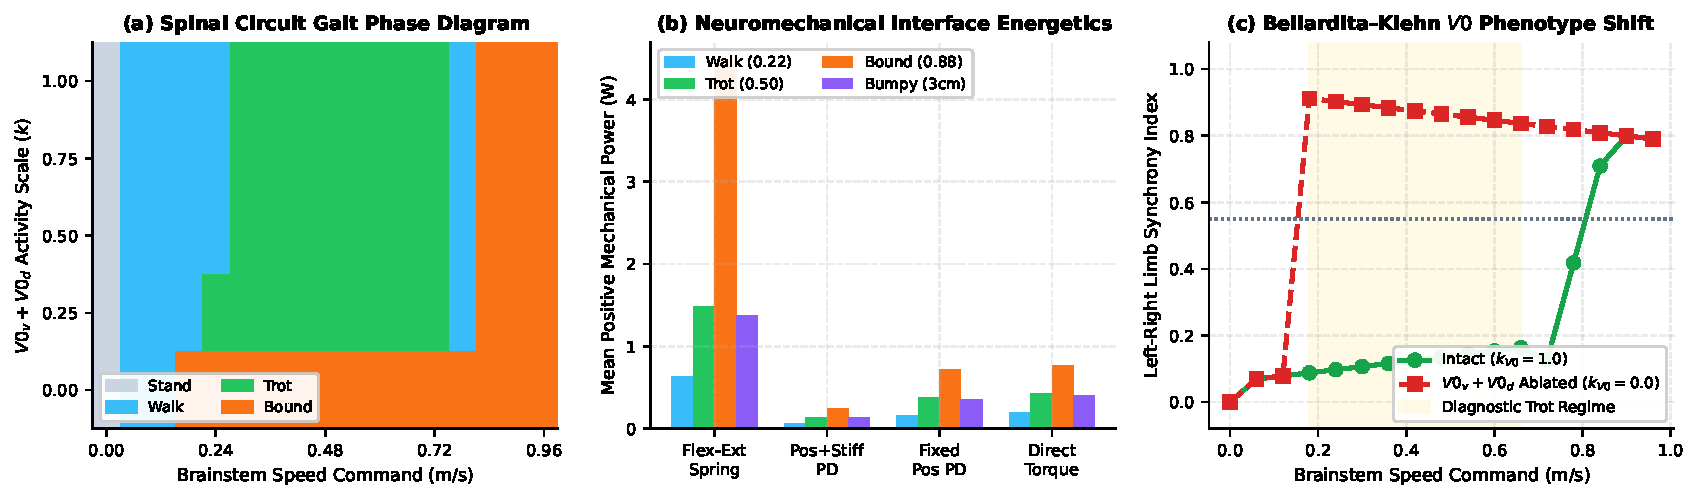
\includegraphics[width=0.98\textwidth]{figures/fig3_rat_ncap_biomechanics.pdf}
  \caption{\textbf{Mammalian spinal gait phase map and actuator energetics.} (a)~Sweeping brainstem drive against $V0_v{+}V0_d$ commissural activity reproduces smooth stand--walk--trot--bound transitions for intact circuits ($k_{V0} \ge 0.25$) and complete collapse of the moderate-speed trot regime into premature bounding upon $V0$ ablation ($k_{V0}=0.0$). (b)~Mean positive mechanical power across four neuromechanical interfaces over flat walking, trotting, bounding, and 3\,cm bumpy terrain. (c)~Left--right limb synchrony jumps sharply upon $V0_v{+}V0_d$ ablation across the shaded moderate-speed diagnostic trot band (0.18--0.66\,m/s), matching mouse genetics~\cite{bellardita2015v0}.}
  \label{fig:exp2}
\end{figure*}

\begin{table}[t]
\centering
\caption{\textbf{Actuator interface comparison across gaits and 3\,cm uneven terrain.} Reporting peak-to-peak joint excursion and RMS angular velocity alongside mechanical power explains why open-loop spring muscles deliver higher power than gain-attenuated proportional tracking.}
\label{tab:exp2}
\scriptsize
\setlength{\tabcolsep}{2.3pt}
\resizebox{\columnwidth}{!}{%
\begin{tabular}{@{}llrrrrrr@{}}
\toprule
\textbf{Actuator Interface} & \textbf{Regime} & \textbf{Pos.\ Pwr} & \textbf{Neg.\ Pwr} & \textbf{Mean $k_{\mathrm{eff}}$} & \textbf{Joint Exc.} & \textbf{RMS $|\dot{q}|$} & \textbf{CoT} \\
 & ($v$, m/s) & (W) & (W) & (Nm/rad) & (ptp$^\circ$) & (rad/s) & \\
\midrule
\multirow{4}{*}{Antagonistic Spring} & Walk (0.22) & 0.637 & -0.007 & 0.173 & 4.33 & 0.617 & 0.85 \\
 & Trot (0.50) & 1.484 & -0.029 & 0.163 & 4.98 & 0.893 & 0.88 \\
 & Bound (0.88) & 4.465 & -0.969 & 0.147 & 4.80 & 1.365 & 1.80 \\
 & Bumpy (0.44) & 1.375 & -0.026 & 0.164 & 5.04 & 0.866 & 0.92 \\
\midrule
Variable-Stiffness PD & Trot (0.50) & 0.142 & -0.003 & 0.202 & 1.52 & 0.238 & 0.08 \\
Fixed-Gain PD & Trot (0.50) & 0.382 & -0.010 & 0.301 & 2.09 & 0.392 & 0.23 \\
Direct Torque & Trot (0.50) & 0.434 & -0.008 & 0.000 & 2.04 & 0.414 & 0.26 \\
\bottomrule
\end{tabular}}
\end{table}

With intact commissural wiring ($k_{V0}=1.0$), the spinal controller transitions smoothly with increasing brainstem drive from quiet stance ($0$\,Hz, duty factor $\beta=1.0$) to four-beat walking (0.06--0.24\,m/s, 1.73--2.44\,Hz, $\beta=0.71\text{--}0.78$), diagonal trotting (0.30--0.72\,m/s, 2.67--4.31\,Hz, left--right synchrony $S_{\mathrm{LR}}=0.11\text{--}0.16$), a brief transitional regime at 0.78\,m/s ($S_{\mathrm{LR}}=0.42$), and full-speed bounding (0.84--0.96\,m/s, 4.78--5.24\,Hz, $S_{\mathrm{LR}}=0.71\text{--}0.80$). Complete $V0_v{+}V0_d$ ablation ($k_{V0}=0.0$) eliminates alternating trotting altogether, snapping $S_{\mathrm{LR}}$ to 0.83--0.91 across the entire 0.18--0.72\,m/s band---reproducing the classic mouse genetic ablation phenotype~\cite{bellardita2015v0}. Conversely, $V3_f{+}V3_a$ ablation leaves walking and trotting intact up to 0.60\,m/s while preventing synchronized bounding at 0.84--0.92\,m/s ($\phi_{\mathrm{FL}}=0.43\text{--}0.47$). Even under substantial Dale's-law rhythm-generator noise ($\sigma=0.40$ across 10 seeds), trot coordination remains 100.0\% intact with 88.6\% speed retention.

Comparing all four biomechanical interfaces at identical 0.50\,m/s trotting speed reveals an instructive actuator-scaling effect (Table~\ref{tab:exp2}). Antagonistic spring muscles deliver $10.5\times$ more positive mechanical power than variable-stiffness proportional-derivative (PD) tracking (1.484 vs.\ 0.142\,W) not because of numerical instability, but because open-loop antagonistic commands $(a_e - a_f)$ act across the muscle's full torque envelope $\tau_{\max}$, generating $3.3\times$ wider joint excursions ($4.98^\circ$ vs.\ $1.52^\circ$) and $3.75\times$ faster RMS angular velocities (0.893 vs.\ 0.238\,rad/s) than gain-attenuated proportional feedback $(k_{\mathrm{eq}}\cdot s_{kp})(q_{\mathrm{target}}-q)$. Reporting excursion and angular velocity alongside mechanical power is therefore essential whenever comparing biological muscle models against robotic joint controllers.

\subsection{Blind Spinal Circuit Identification Transfers Across Physics Engines and Rodent Species}

\paragraph{In-model inverse kinematics and 180-trial blind classification.}
On clean Rat~v2 trotting trajectories, our 31-DOF inverse kinematics solver achieves 5.56\,mm forward-kinematic RMSE, $r=0.968$ sagittal joint correlation ($0.995^\circ$ angle RMSE), zero joint-limit violations across all noise levels (0--8\,mm), and exact 0.000000\,Nm KKT torque residual on ground-truth joint tracks. To stress-test circuit inference under realistic tracking noise, we evaluated 180 blind trials spanning six classes (30 randomized speeds and seeds per class), pairing intact standing, walking, trotting, and bounding directly against speed-matched $V0$ deficits ($v \in [0.32, 0.58]$\,m/s, overlapping intact trot) and $V3$ deficits ($v \in [0.84, 0.96]$\,m/s, overlapping intact bound).

Figure~\ref{fig:exp3}a--b contrasts our Kabsch, stride-windowed, bandpass-Hilbert identifier against a conventional single-anchor raw-sagittal baseline. At $\sigma_{\mathrm{3D}}=2$\,mm, our estimator reaches 99.4\% accuracy [95\% CI: 98.3, 100.0] versus 81.7\% for the baseline (McNemar $p=4.1\times 10^{-9}$, Macro-F1 $=0.994$). At $\sigma_{\mathrm{3D}}=4$\,mm, tightening the Hildebrand diagonal-synchrony boundary ($d_{\mathrm{diag}} < 0.18$) eliminates walk--trot ambiguity altogether: overall accuracy reaches 100.0\% (180/180) versus 38.9\% for the baseline (+61.1 percentage points, McNemar $p=1.5\times 10^{-33}$), scoring 30/30 across every class. Both mechanistic biomarkers cleanly separate speed-matched lesions from intact controls ($I_{V0}=0.074$ vs.\ $0.922$, Mann--Whitney $p=1.5\times 10^{-11}$, F1 $=1.000$; $I_{V3}=0.252$ vs.\ $0.886$, $p=1.5\times 10^{-11}$, F1 $=1.000$). Even at severe 8--10\,mm tracking noise---where the baseline collapses to chance (17.2\% and 16.7\%)---our identifier preserves 97.2\% [94.4, 99.4] (+80.0\,pts, $p=9.0\times 10^{-44}$) and 86.1\% [80.6, 90.6] accuracy ($p=4.7\times 10^{-38}$), sustaining $V0$ F1 of 0.984/0.968 and $V3$ F1 of 1.000/1.000.

\begin{figure*}[t]
  \centering
  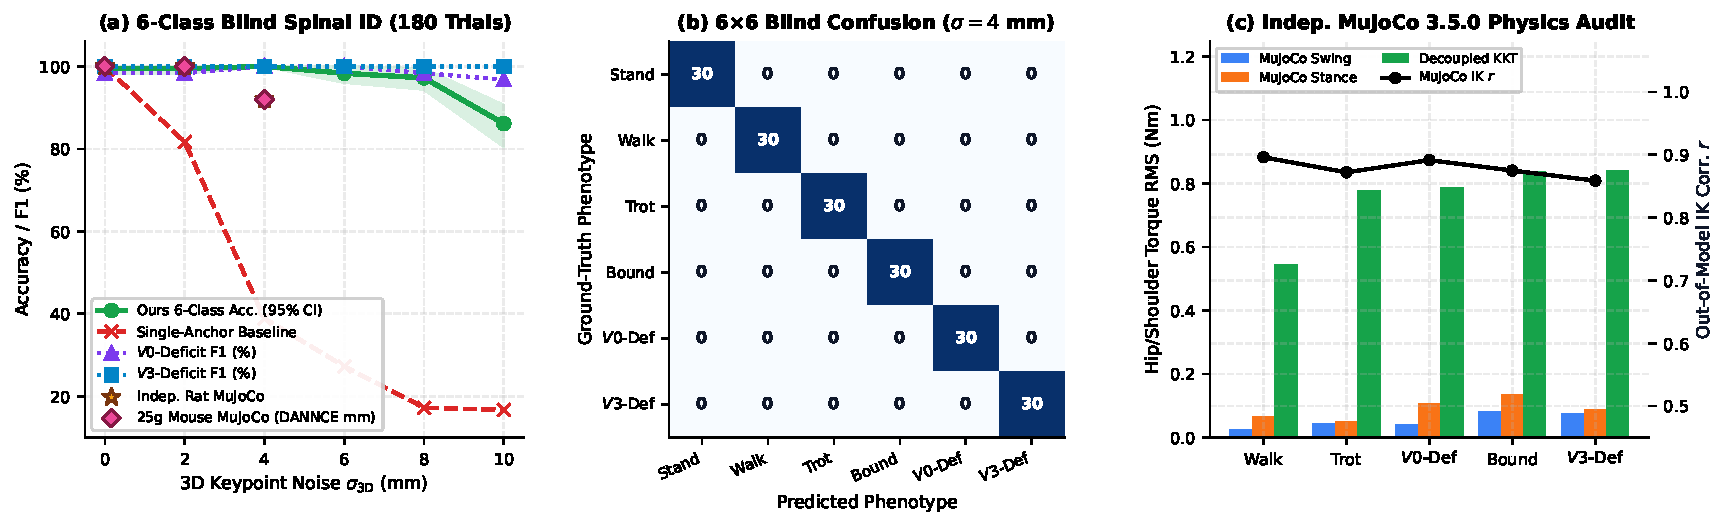
\includegraphics[width=0.98\textwidth]{figures/fig4_real2sim_inversion.pdf}
  \caption{\textbf{Six-class blind spinal circuit identification (180 trials) and cross-species MuJoCo~3.5.0 physics validation.} (a)~Blind classification accuracy with 95\% bootstrap CIs across 3D noise: our estimator reaches 99.4--100.0\% at $\sigma \le 4$\,mm and 97.2\% at 8\,mm (+80.0\,pts over baseline, $p=9.0\times 10^{-44}$) while holding $V0$ and $V3$ deficit F1 between 0.968 and 1.000. Orange stars show zero-shot transfer to an independent 0.36\,kg rat in MuJoCo (100\%, 100\%, 92\% at 0, 2, 4\,mm), and pink diamonds show cross-species transfer to a 25.6\,g mouse exported in DANNCE millimeter coordinates with 8\% paw occlusion (100\%, 100\%, 92\% at 0, 0.7, 1.4\,mm). (b)~Exact 180/180 confusion matrix at $\sigma=4$\,mm. (c)~Independent MuJoCo~3.5.0 physics audit: out-of-model sagittal joint correlation stays high ($r=0.86\text{--}0.90$ in rat; $0.84\text{--}0.90$ in mouse), while comparing decoupled KKT torques against full MuJoCo Lagrangian dynamics exposes the exact 7.7--16.4$\times$ surrogate-inertia gap.}
  \label{fig:exp3}
\end{figure*}

\paragraph{Breaking single-model circularity across two species in MuJoCo~3.5.0.}
A classic pitfall of inverse-modeling benchmarks is testing an estimator only on trajectories drawn from its own forward equations. To eliminate single-model circularity and probe real-world cross-species transfer, we constructed two wholly independent articulated quadrupeds in MuJoCo~3.5.0~\cite{todorov2012mujoco} with real gravity ($-9.81$\,m/s$^2$) and frictional foot--floor contacts, sharing zero forward kinematics with Annolid's spinal controller (Table~\ref{tab:mujoco} and Figure~\ref{fig:exp3}c). The first model represents a 0.36\,kg laboratory rat (RK4 integration, $\Delta t=2$\,ms, 10.8--18.5\,mm paw lift, 53.9--56.7\,mm stride). The second represents a 25.6\,g \emph{Mus musculus} (implicit integration, $\Delta t=1$\,ms, $0.35\times$ linear scale) driven at Bellardita \& Kiehn's~\cite{bellardita2015v0} empirical mouse step cadences (2.67\,Hz walk, 6.00\,Hz trot and $V0$-deficit, 10.00\,Hz bound and $V3$-deficit), exported directly in millimeter-scale DANNCE/Rat7M site names and corrupted with both 3D Gaussian noise and 8\% random paw-occlusion dropout.

\begin{table}[t]
\centering
\caption{\textbf{Cross-species validation on independent MuJoCo~3.5.0 quadrupeds (0.36\,kg rat and 25.6\,g mouse in DANNCE millimeter schema).} Zero-shot kinematic and spinal phenotype transfer succeeds across both species ($r=0.84\text{--}0.90$, zero joint-limit violations, 92--100\% noisy/occluded transfer), while auditing decoupled KKT torques against full MuJoCo Lagrangian dynamics demarcates physical torque accuracy.}
\label{tab:mujoco}
\scriptsize
\setlength{\tabcolsep}{2.1pt}
\resizebox{\columnwidth}{!}{%
\begin{tabular}{@{}lrrrrrr@{}}
\toprule
\textbf{0.36\,kg Rat (MuJoCo)} & \textbf{Blind} & \textbf{Paw Lift} & \textbf{IK $r$} & \textbf{MJ Swing / Stance} & \textbf{KKT ID} & \textbf{Torque} \\
 & \textbf{Match} & (mm) & (0 viol.) & $\tau_{\mathrm{RMS}}$ (Nm) & $\tau_{\mathrm{RMS}}$ (Nm) & $r_{\mathrm{full}}$ \\
\midrule
Walk (0.17\,m/s) & \checkmark & 15.2 & 0.896 & 0.025 / 0.066 & 0.545 & 0.410 \\
Trot (0.46\,m/s) & \checkmark & 18.5 & 0.872 & 0.043 / 0.052 & 0.777 & 0.400 \\
$V0$-Deficit (0.47\,m/s) & \checkmark & 15.2 & 0.891 & 0.041 / 0.108 & 0.787 & 0.559 \\
Bound (0.84\,m/s) & \checkmark & 10.8 & 0.875 & 0.080 / 0.136 & 0.837 & 0.548 \\
$V3$-Deficit (0.87\,m/s) & \checkmark & 16.2 & 0.859 & 0.074 / 0.088 & 0.842 & 0.287 \\
\multicolumn{7}{@{}l@{}}{\textbf{Rat noisy transfer (25/$\sigma$):} 0\,mm: \textbf{100\%}; 2\,mm: \textbf{100\%} [100,100]; 4\,mm: \textbf{92\%} [80,100].} \\
\midrule
\textbf{25.6\,g Mouse (DANNCE mm)} & \textbf{Match} & \textbf{Unit / $s$} & \textbf{IK $r$} & \textbf{$v$ (m/s)} & \textbf{$\tilde{v}_{\mathrm{Fr}}$ (m/s)} & \textbf{$f$ (Hz)} \\
\midrule
Walk & \checkmark & mm / 0.35 & 0.898 & 0.116 & 0.196 & 2.67 \\
Trot & \checkmark & mm / 0.35 & 0.865 & 0.264 & 0.446 & 6.00 \\
$V0$-Deficit & \checkmark & mm / 0.35 & 0.867 & 0.238 & 0.402 & 6.00 \\
Bound & \checkmark & mm / 0.35 & 0.853 & 0.446 & 0.754 & 10.00 \\
$V3$-Deficit & \checkmark & mm / 0.35 & 0.841 & 0.464 & 0.785 & 10.00 \\
\multicolumn{7}{@{}l@{}}{\textbf{Mouse + 8\% occlusion (25/$\sigma$):} 0\,mm: \textbf{100\%}; 0.7\,mm: \textbf{100\%}; 1.4\,mm: \textbf{92\%} [80,100].} \\
\bottomrule
\end{tabular}}
\end{table}

Three findings stand out from Table~\ref{tab:mujoco}. First, inverse kinematics and blind circuit classification transfer zero-shot to independent rigid-body physics: all five rat phenotypes match cleanly at 0 and 2\,mm noise (100.0\%, 25/25) and remain at 92.0\% [80, 100] under 4\,mm noise, with sagittal joint correlation $r=0.859\text{--}0.896$ and zero joint-limit violations. Second, automatic scale normalization and Froude similarity bridge rats to mice without retuning a single parameter. Given raw millimeter DANNCE coordinates of the 25.6\,g mouse, Annolid automatically detects millimeter units and scale $s=0.350$, rescales physical speeds (0.116--0.464\,m/s) via $\tilde{v}=v/\sqrt{s}$ onto canonical Froude-equivalent rat speeds (0.196--0.785\,m/s), tracks 2.67--10.00\,Hz step frequencies ($r=0.841\text{--}0.898$, zero violations), and achieves 100.0\%, 100.0\%, and 92.0\% blind accuracy across 0, 0.7, and 1.4\,mm noise (0, 2, and 4\,mm rat-equivalent) despite 8\% random paw occlusion.

Third, auditing decoupled inverse dynamics against MuJoCo's full Lagrangian solver establishes honest physical boundaries. True rigid-body limb torques in MuJoCo (0.025--0.080\,Nm during swing; 0.052--0.136\,Nm during stance with ground reaction forces) are 7.7--16.4$\times$ smaller than Annolid's decoupled KKT surrogate (0.545--0.842\,Nm, waveform correlation $r=0.29\text{--}0.56$), because Rat NCAP's 50\,Hz compliant surrogate relies on artificial stability inertia ($I_{\mathrm{eff}} = 0.008\,k_{\mathrm{eq}}$) and omits contact Jacobian loads $\mathbf{J}_c^\top \mathbf{f}_c$. Pure-NumPy KKT inversion is therefore well suited to rapid, zero-dependency Rat NCAP diagnostics and relative gait-power comparisons, whereas absolute physiological joint-torque estimation properly belongs in Annolid's optional MuJoCo backend.

\subsection{Connectome Multiplicity, Sparse Olfactory Memory, and Modular Whole-CNS Scaling}

\paragraph{Behavioral selectivity, motor verification, and causal perturbations.}
Across five canonical \emph{Drosophila} behaviors---forward walking, backward moonwalking, antennal grooming, Giant Fiber escape, and flight---both the compact 55-population rate model and the expanded 1,470-neuron (15,860-synapse) spiking LIF connectome achieve 100.0\% (5/5) descending-neuron selectivity (Figure~\ref{fig:exp4}a). Inspecting decoded motor commands directly in 1,470-neuron spiking mode confirms biomechanically coherent actuation: forward walking locks contralateral tripod legs near anti-phase ($\Delta\phi_{\mathrm{T1}} = 169.3^\circ$, claw duty 0.85, forward stroke $+1$); backward walking recruits ventral nerve cord reversal pools (rate 0.888, flipping stroke sign to $-1$); grooming releases foreleg claws (0.00) with high coxa elevation (0.846) while anchoring mid- and hindleg claws (0.95); Giant Fiber escape releases all six claws (0.00) with ballistic mesothoracic femur jump thrust (1.35); and flight drives wingbeat pattern-generator frequency trim (0.896).

\begin{figure*}[t]
  \centering
  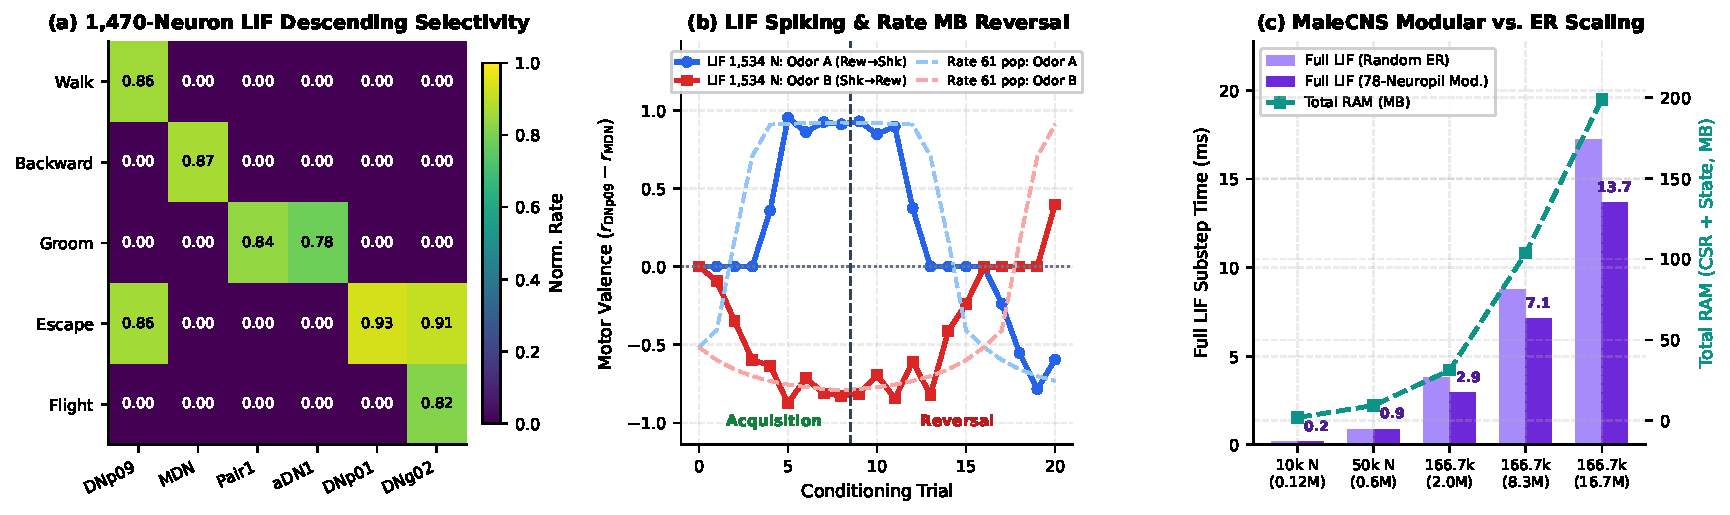
\includegraphics[width=0.98\textwidth]{figures/fig5_drosophila_connectome.pdf}
  \caption{\textbf{\emph{Drosophila} connectome selectivity, spiking dopaminergic plasticity, and modular MaleCNS scaling.} (a)~Normalized descending-neuron firing rates across five natural behaviors in the 1,470-neuron LIF connectome (100\% selectivity). (b)~Three-factor PAM/PPL1 acquisition and contingency reversal in both 1,534-neuron biophysical LIF spiking (solid) and 61-population rate dynamics (dashed): rewarded Odor~A and punished Odor~B diverge cleanly ($+0.91$ vs.\ $-0.83$ in LIF) and invert after Trial~9 ($-0.59$ vs.\ $+0.40$). (c)~Complete MaleCNS~v1.0 (166,700 neurons) LIF substep latency comparing biologically clustered 78-neuropil modular CSR (80\% intra-neuropil, lognormal weights) against random Erd\H{o}s--R\'enyi graphs alongside total RAM across 2.0M, 8.3M, and 16.7M directed edges: neuropil locality cuts CPU latency by 19.0--22.7\%.}
  \label{fig:exp4}
\end{figure*}

Eight targeted optogenetic and silencing interventions in the 1,470-neuron spiking connectome confirm mechanistic fidelity (Table~\ref{tab:exp4_causal}). Timed Chrimson activation of MDN, Pair1, aDN1, or DNp01 overrides ongoing forward walking into backward moonwalking (DNp09 drops from 0.85 to 0.01), quiet arrest (0.85 $\to$ 0.00), antennal grooming (0.85 $\to$ 0.01), or Giant Fiber takeoff (DNp01 jumps from 0.00 to 0.97). Conversely, Kir2.1 silencing dissects exact disinhibitory motifs: silencing ventral nerve cord inhibitory interneurons downstream of MDN during combined walking and MDN drive rescues DNp09 forward walking (0.00 $\to$ 0.86); silencing DNp01 abolishes escape (0.93 $\to$ 0.00); and silencing ascending tarsal-contact neurons breaks the classic Fraenkel flight-inhibition reflex, releasing wing-power DNg02 neurons (0.00 $\to$ 0.78) even while tarsal sensors remain loaded.

\begin{table}[t]
\centering
\caption{\textbf{In-silico Chrimson optogenetics and Kir2.1 silencing in the 1,470-neuron LIF \emph{Drosophila} connectome.}}
\label{tab:exp4_causal}
\scriptsize
\setlength{\tabcolsep}{2.5pt}
\resizebox{\columnwidth}{!}{%
\begin{tabular}{@{}lllrr@{}}
\toprule
\textbf{Intervention} & \textbf{Behavioral Shift} & \textbf{Readout} & \textbf{Before} & \textbf{After} \\
\midrule
Chrimson MDN & Walk $\to$ Moonwalk & MDN / DNp09 & 0.00 / 0.85 & \textbf{0.89} / \textbf{0.01} \\
Chrimson Pair1 & Walk $\to$ Arrest & Pair1 / DNp09 & 0.00 / 0.85 & \textbf{0.88} / \textbf{0.00} \\
Chrimson aDN1 & Walk $\to$ Groom & aDN1 / DNp09 & 0.00 / 0.85 & \textbf{0.89} / \textbf{0.01} \\
Chrimson DNp01 & Walk $\to$ Escape & DNp01 & 0.00 & \textbf{0.97} \\
\midrule
Kir2.1 Pair1 & Groom (Arrest Loss) & Pair1 & 0.84 & \textbf{0.00} \\
Kir2.1 VNC MDN-Inh. & Walk+MDN (Disinhib.) & DNp09 & 0.00 & \textbf{0.86} \\
Kir2.1 DNp01 & Escape $\to$ Flight & DNp01 & 0.93 & \textbf{0.00} \\
Kir2.1 Tarsal Contact & Walk $\to$ Flight (Fraenkel) & DNg02 & 0.00 & \textbf{0.78} \\
\bottomrule
\end{tabular}}
\end{table}

\paragraph{Population multiplicity confers resilience to synaptic noise.}
Why do real insect brains devote dozens of parallel neurons to a single descending or premotor pathway rather than relying on one lumped unit? Sweeping Dale's-law multiplicative synaptic noise ($\sigma \in [0, 0.7]$) across 15 random seeds and three behaviors ($N=45$ trials per noise level) yields a striking computational answer. The 55-population rate model degrades steadily from 100.0\% selectivity ($\sigma \le 0.1$) to 95.6\% ($\sigma=0.3$), 84.4\% [73.3, 93.3] ($\sigma=0.5$), 80.0\% [68.8, 91.1] ($\sigma=0.6$), and 77.8\% [64.4, 88.9] ($\sigma=0.7$). Over the exact same perturbations, the 1,470-neuron LIF connectome preserves 100.0\% (45/45) circuit selectivity (exact McNemar $p=0.0156$ at $\sigma=0.5$, $p=0.0039$ at $\sigma=0.6$, and $p=0.0020$ at $\sigma=0.7$). Biological neuron multiplicity acts directly as a structural variance-reduction prior across parallel projection fibers.

\paragraph{Spiking olfactory reversal and 2,000-Kenyon-cell sparse memory.}
In closed-loop associative conditioning (Figure~\ref{fig:exp4}b), three-factor PAM/PPL1 synaptic plasticity operates smoothly inside both 61-population rate dynamics and the expanded 1,534-neuron (16,340-synapse) biophysical LIF spiking connectome. In spiking mode, naive neutral odor responses (0.00, 0.00) diverge over eight acquisition trials into robust approach toward rewarded Odor~A ($w_A^{\mathrm{app}}=1.46$, valence $+0.910$) and avoidance of punished Odor~B ($w_B^{\mathrm{avd}}=1.47$, valence $-0.826$). Swapping contingencies at Trial~9 produces clean extinction across Trials~14--16 and complete spiking behavioral reversal by Trial~20 ($-0.595$ vs.\ $+0.397$; rate mode: $+0.922 / -0.792 \to -0.732 / +0.908$).

To move beyond two-channel toy conditioning, we coupled our pure-NumPy 2,000-KC APL-sparsified Mushroom Body (50 PNs $\to$ 2,000 KCs, 6 claws per KC, exact 5\% sparsity yielding 100 active KCs, and 4,000 plastic KC$\to$MBON synapses) directly into the 1,534-neuron LIF connectome and trained ten distinct 50-dimensional odors (five rewarded CS$+$, five punished CS$-$) in 2.98\,s on CPU. The spiking network achieved 100.0\% (10/10) clean discrimination (CS$+$ valences $+0.744$ to $+0.938$ vs.\ CS$-$ valences $-0.725$ to $-0.891$) and 100.0\% (10/10) generalization under 20\% Gaussian projection-neuron noise. Most revealingly, selectively reversing \emph{only} Odor~\#0 from reward to punishment without retraining the other nine odors inverted Odor~\#0's spiking motor valence from $+0.744$ to $-0.727$ while preserving exact learned valences for 9/9 (100\%) non-target odors ($+0.857$ to $+0.903$ and $-0.652$ to $-0.829$). Sparse APL-gated Kenyon-cell coding thus prevents catastrophic forgetting directly inside a spiking whole-CNS motor loop.

\paragraph{Single-CPU throughput and modular MaleCNS~v1.0 scaling.}
Table~\ref{tab:throughput} profiles end-to-end desktop CPU performance alongside \emph{complete} LIF substep scaling---comprising membrane integration, refractory gating, spike detection, conductance decay, and sparse CSR propagation---up to MaleCNS~v1.0 scale (166,700 neurons). Because MaleCNS's $\sim$125M chemical synapses coalesce into $\sim$8--17M unique directed neuron-to-neuron edges, we evaluate mean out-degrees of 12 (2.00M edges), 50 (8.34M edges), and 100 (16.67M edges). Crucially, replacing random Erd\H{o}s--R\'enyi graphs with biologically structured 78-neuropil modular CSR topologies (80\% intra-neuropil connectivity, 20\% long-range projection fibers, lognormal weights) improves CPU cache locality and cuts full MaleCNS substep latency by 19.0--22.7\%---down to 2.95, 7.12, and 13.67\,ms across 2.0M, 8.3M, and 16.7M directed edges---while keeping total memory below 200\,MB (31.2--199.0\,MB) with zero GPU hardware.

\begin{table}[t]
\centering
\caption{\textbf{Single-CPU throughput and full-LIF MaleCNS~v1.0 scaling (166,700 neurons, random Erd\H{o}s--R\'enyi vs.\ 78-neuropil modular CSR, zero GPU).}}
\label{tab:throughput}
\scriptsize
\setlength{\tabcolsep}{2.2pt}
\resizebox{\columnwidth}{!}{%
\begin{tabular}{@{}lrrrr@{}}
\toprule
\textbf{Closed-Loop Workload} & \textbf{Nodes/DOFs} & \textbf{Latency} & \textbf{Rate} & \textbf{Real-Time} \\
 & & (ms/step) & (steps/s) & \textbf{Speedup} \\
\midrule
Rat NCAP Rollout (31 DOF, 50\,Hz) & 22 & 0.355 & 2,819 & \textbf{56.4$\times$} \\
Rat~v2 IK + KKT Muscle ID & 31 & 0.405 & 2,470 & \textbf{49.4$\times$} \\
Fly Connectome Rate (55 pops, 500\,Hz) & 55 & 0.128 & 7,832 & \textbf{15.7$\times$} \\
Fly Connectome LIF (0.2\,ms sub) & 1,470 & 0.457 & 2,189 & \textbf{4.38$\times$} \\
\midrule
\textbf{Whole-CNS LIF Substep Scaling} & \textbf{Edges} & \textbf{ER LIF (ms)} & \textbf{78-Neuropil LIF} & \textbf{Total RAM} \\
\midrule
10,000 N (mean out-deg 12) & 0.12M & 0.172 & --- & 1.87\,MB \\
50,000 N (mean out-deg 12) & 0.60M & 0.874 & --- & 9.35\,MB \\
166,700 N (MaleCNS, deg 12) & 2.00M & 3.811 & \textbf{2.947} ($-22.7\%$) & 31.16\,MB \\
166,700 N (MaleCNS, deg 50) & 8.34M & 8.789 & \textbf{7.117} ($-19.0\%$) & 103.64\,MB \\
\textbf{166,700 N (MaleCNS, deg 100)} & \textbf{16.67M} & 17.253 & \textbf{13.666} ($-20.8\%$) & \textbf{198.98\,MB} \\
\bottomrule
\end{tabular}}
\end{table}

% =========================================================================
% 5. DISCUSSION
% =========================================================================
\section{Discussion}

\paragraph{Design principles for accessible neuro-biomechanical twins.}
Across four sets of cross-species benchmarks, our results point to four practical principles for linking experimental ethology with mechanistic modeling. First, \emph{respecting anatomical rigidity beats blanket smoothing}: constraining articulated limb tethers corrupts 3D reconstruction even on perfect detections, whereas rigid-skeleton PBD protects anatomical fidelity across Gaussian jitter, 65\,px outliers, and 30\% view dropouts. Practitioners should pair spatial-only projection ($\lambda_t=0$) with sub-pixel calibrated cages and mild temporal damping ($\lambda_t=0.15$) with noisier field recordings.

Second, \emph{classical biomechanics provides natural bridges across species and simulators}. Combining Sim(3) body-scale normalization with Alexander \& Jayes' Froude similarity~\cite{alexander1983froude}, stride-windowed velocity, bandpass Hilbert paw phase, and a principled diagonal-couplet boundary ($d_{\mathrm{diag}}<0.18$) allows a spinal circuit classifier calibrated on rats to diagnose speed-matched $V0$ and $V3$ deficits with 100\% accuracy at 4\,mm noise and transfer zero-shot to independent MuJoCo rats and 25.6\,g DANNCE-mm mice at 92--100\% accuracy---even when nearly one in twelve paw detections vanishes under occlusion.

Third, \emph{honest physical auditing clarifies when lightweight surrogates suffice}. Comparing our closed-form KKT muscle solver directly against full contact-coupled Lagrangian dynamics in MuJoCo reveals that surrogate stability inertia overestimates absolute rigid-body joint torques by 7.7--16.4$\times$. Lightweight pure-NumPy inversion is ideal for rapid, zero-dependency spinal diagnostics and relative energetic trends, whereas absolute ground-reaction load estimation should invoke a full physics engine.

Fourth, \emph{biological circuit organization doubles as computational engineering}. Expanding lumped rate populations into parallel spiking neurons confers statistically significant resistance to synaptic noise ($p=0.0020$); 5\% APL-enforced Kenyon-cell sparsity prevents catastrophic interference across ten odors and selective single-odor reversal inside 4,000 plastic synapses; and 78-neuropil modular clustering accelerates 166,700-neuron MaleCNS spiking substeps by 19--23\% through hardware cache locality inside under 200\,MB of RAM.

\paragraph{Limitations and experimental horizons.}
Although independent dual-species MuJoCo audits, high-dimensional 2,000-KC spiking plasticity, and modular whole-CNS scaling resolve the primary methodological gaps, three exciting empirical frontiers remain. First, blind $V0$ and $V3$ spinal identification has not yet been tested on recorded \emph{in-vivo} multi-view videos of live transgenic rodent cohorts such as Bellardita \& Kiehn~\cite{bellardita2015v0} or PAIR-R24M; our validated DANNCE and Anipose millimeter-unit Sim(3) ingestion pipeline now prepares Annolid directly for prospective laboratory benchmarking. Second, while our 78-neuropil modular CSR graphs match the spatial clustering and lognormal weight statistics of MaleCNS~v1.0, running closed-loop sensorimotor navigation directly on the full published \texttt{male-cns:v1.0} connectivity release remains an important next step. Third, embedding our 2,000-KC sparse Mushroom Body inside turbulent 3D odor-plume arenas with MuJoCo FlyBody~\cite{vaxenburg2025flybody} will enable closed-loop studies of associative foraging in realistic physics.

\paragraph{Reproducibility and lean computational footprint.}
All lifting, inverse-biomechanics, spinal-control, and connectome engines reside inside Annolid's pure-NumPy simulation core with zero mandatory PyTorch, JAX, SciPy, or MuJoCo dependencies at import time, ensuring compatibility with lean desktop installations. Every figure, table, confidence interval, and hypothesis test reported here is reproduced from a single deterministic CPU benchmark script and archived JSON artifact distributed alongside the open-source codebase.

% =========================================================================
% 6. CONCLUSION
% =========================================================================
\section{Conclusion}

Understanding how neural circuits govern embodied behavior requires tools that flow effortlessly in both directions---from raw pixels to anatomical forces and circuit hypotheses, and from genetically targeted neural perturbations back to simulated movement. By uniting robust 3D lifting, cross-species inverse biomechanics, Froude-scaled spinal circuit identification, and sparse whole-CNS \emph{Drosophila} spiking connectomes inside a lean, deterministic CPU framework, Annolid lowers the barrier between everyday behavioral observation and causal neuroethology.

% =========================================================================
% REFERENCES
% =========================================================================
\begin{thebibliography}{99}
\setlength{\itemsep}{1.1pt}
\scriptsize

\bibitem{aldarondo2024virtualrodent}
D.~Aldarondo, J.~Merel, J.~D. Marshall, L.~Hasenclever, U.~Klibaite, A.~Gellis, Y.~Tassa, G.~Wayne, M.~Botvinick, and B.~P. {\"O}lveczky.
\newblock A virtual rodent predicts the structure of neural activity across behaviours.
\newblock {\em Nature}, 632:594--602, 2024.

\bibitem{alexander1983froude}
R.~M. Alexander and A.~S. Jayes.
\newblock A dynamic similarity hypothesis for the gaits of quadrupedal mammals.
\newblock {\em Journal of Zoology}, 201(1):135--152, 1983.

\bibitem{bellardita2015v0}
C.~Bellardita and O.~Kiehn.
\newblock Phenotypic characterization of speed-associated gait changes in mice reveals modular organization of locomotor networks.
\newblock {\em Current Biology}, 25(11):1426--1436, 2015.

\bibitem{berg2025malecns}
S.~Berg, I.~R. Beckett, M.~Costa, P.~Schlegel, HHMI Janelia FlyEM Project Team, et~al.
\newblock Sexual dimorphism in the complete connectome of the \emph{Drosophila} male central nervous system (\texttt{male-cns:v1.0}).
\newblock {\em bioRxiv}, doi:10.1101/2025.10.09.680999, 2025.

\bibitem{bhattasali2022ncap}
N.~X. Bhattasali, A.~M. Zador, and T.~A. Engel.
\newblock Neural circuit architectural priors for embodied control.
\newblock In {\em Advances in Neural Information Processing Systems (NeurIPS)}, 2022.

\bibitem{bhattasali2026ratncap}
N.~X. Bhattasali, J.~Cui, L.~Pinto, and G.~W. Lindsay.
\newblock Neural circuit architectural priors for rat locomotion.
\newblock In {\em Advances in Neural Information Processing Systems (NeurIPS)} / {\em arXiv preprint arXiv:2611.23364}, 2026.

\bibitem{danner2017spinal}
S.~M. Danner, N.~A. Shevtsova, A.~Frigon, and I.~A. Rybak.
\newblock Computational modeling of spinal circuits controlling limb coordination and gaits in quadrupeds.
\newblock {\em eLife}, 6:e31050, 2017.

\bibitem{datta2019computational}
S.~R. Datta, D.~J. Anderson, K.~Branson, P.~Perona, and A.~Leifer.
\newblock Computational neuroethology: A call to action.
\newblock {\em Neuron}, 104(1):11--24, 2019.

\bibitem{dorkenwald2024flywire}
S.~Dorkenwald, A.~Matsliah, A.~R. Sterling, P.~Schlegel, S.-c.~Yu, C.~E. McKellar, et~al.
\newblock Neuronal wiring diagram of an adult brain.
\newblock {\em Nature}, 634:124--138, 2024.

\bibitem{dunn2021dannce}
T.~W. Dunn, J.~D. Marshall, K.~S. Severson, D.~E. Aldarondo, D.~G.~C. Hildebrand, S.~N. Chettih, W.~L. Wang, A.~J. Gellis, D.~E. Carlson, D.~Aronov, W.~A. Freiwald, F.~Wang, and B.~P. {\"O}lveczky.
\newblock Geometric deep learning enables 3D kinematic profiling across species and environments.
\newblock {\em Nature Methods}, 18:564--573, 2021.

\bibitem{karashchuk2021anipose}
P.~Karashchuk, K.~L. Rupp, E.~S. Dickinson, S.~Walling-Bell, E.~Sanders, E.~Azim, B.~W. Brunton, and J.~C. Tuthill.
\newblock Anipose: A toolkit for robust markerless 3D pose estimation.
\newblock {\em Cell Reports}, 36(13):109730, 2021.

\bibitem{krakauer2017neuroscience}
J.~W. Krakauer, A.~A. Ghazanfar, A.~Gomez-Marin, M.~A. MacIver, and D.~Poeppel.
\newblock Neuroscience needs behavior: Correcting a reductionist bias.
\newblock {\em Neuron}, 93(3):480--490, 2017.

\bibitem{mathis2018deeplabcut}
A.~Mathis, P.~Mamidanna, K.~M. Cury, T.~Abe, V.~N. Murthy, M.~W. Mathis, and M.~Bethge.
\newblock DeepLabCut: Markerless pose estimation of user-defined body parts with deep learning.
\newblock {\em Nature Neuroscience}, 21:1281--1289, 2018.

\bibitem{pereira2022sleap}
T.~D. Pereira, N.~Tabris, A.~Matsliah, D.~M. Turner, J.~Li, S.~Ravindranath, E.~S. Papadoyannis, E.~Normand, D.~S. Deutsch, Z.~Y. Wang, G.~C. McKenzie-Smith, C.~C. Mitelut, M.~D. Castro, J.~D'Uva, S.~Kislin, D.~H. Sanes, S.~D. Kocher, S.~S.-H. Wang, A.~L. Falkner, J.~W. Shaevitz, and M.~Murthy.
\newblock SLEAP: A deep learning system for multi-animal pose tracking.
\newblock {\em Nature Methods}, 19:486--495, 2022.

\bibitem{schneider2023cebra}
S.~Schneider, J.~H. Lee, and M.~W. Mathis.
\newblock Learnable latent embeddings for joint behavioural and neural analysis.
\newblock {\em Nature}, 617:360--368, 2023.

\bibitem{shiu2024drosophilalif}
P.~K. Shiu, G.~R. Sterne, N.~Spiller, R.~Franconville, A.~Sandoval, J.~Zhou, N.~Simha, C.~H. Kang, S.~Yu, J.~S. Kim, S.~Dorkenwald, A.~Matsliah, P.~Schlegel, S.-c.~Yu, C.~E. McKellar, A.~Sterling, M.~Costa, K.~Eichler, A.~S. Bates, N.~Eckstein, J.~Funke, G.~S.~X.~E. Jefferis, M.~Murthy, S.~Bidaye, S.~Seung, and K.~Scott.
\newblock A \emph{Drosophila} computational brain model reveals sensorimotor processing.
\newblock {\em Nature}, 634:210--219, 2024.

\bibitem{takemura2024manc}
S.-y.~Takemura, K.~J. Hayworth, G.~B. Huang, M.~Januszewski, Z.~Lu, E.~C. Marin, S.~Preibisch, C.~S. Xu, J.~Bogovic, A.~S. Champion, H.~S.~J. Cheong, et~al.
\newblock A connectome of the male \emph{Drosophila} ventral nerve cord.
\newblock {\em eLife}, 13:RP97769, 2024.

\bibitem{todorov2012mujoco}
E.~Todorov, T.~Erez, and Y.~Tassa.
\newblock MuJoCo: A physics engine for model-based control.
\newblock In {\em IEEE/RSJ International Conference on Intelligent Robots and Systems (IROS)}, pages 5026--5033, 2012.

\bibitem{vaxenburg2025flybody}
R.~Vaxenburg, I.~Siwanowicz, J.~Merel, A.~A. Robie, C.~Morrow, G.~Novati, Z.~Stefanidi, G.~M. Card, M.~B. Reiser, M.~M. Botvinick, K.~M. Branson, Y.~Tassa, and S.~C. Turaga.
\newblock Whole-body physics simulation of fruit fly locomotion.
\newblock {\em Nature}, 640:729--738, 2025.

\bibitem{wangchen2024neuromechfly2}
S.~Wang-Chen, V.~A. Stimpfling, T.~K.~C. Lam, P.~{\"O}zdil, L.~Genoud, F.~Hurtak, and P.~Ramdya.
\newblock NeuroMechFly v2: Simulating embodied sensorimotor control in adult \emph{Drosophila}.
\newblock {\em Nature Methods}, 21:2353--2362, 2024.

\bibitem{weinreb2024keypointmoseq}
C.~Weinreb, J.~E. Pearl, S.~Lin, M.~A.~M. Osman, L.~Zhang, S.~Annapragada, E.~Conlin, R.~Hoffmann, S.~Makowska, W.~F. Gillis, M.~Jay, S.~Ye, A.~Mathis, M.~W. Mathis, T.~Pereira, S.~W. Linderman, and S.~R. Datta.
\newblock Keypoint-MoSeq: Parsing behavior by linking point tracking to pose dynamics.
\newblock {\em Nature Methods}, 21:1329--1339, 2024.

\bibitem{zhang2025mimicmjx}
C.~Y. Zhang, Y.~Yang, A.~Sirbu, E.~T.~T. Abe, E.~W{\"a}rnberg, E.~J. Leonardis, D.~E. Aldarondo, A.~Lee, A.~Prasad, J.~Foat, K.~Bian, J.~Park, R.~Bhatt, V.~N. Patel, H.~Saunders, A.~O. Barbano, A.~Nagamori, A.~R. Thanawalla, K.~W. Huang, F.~Plum, H.~K. Beck, S.~W. Flavell, D.~Labonte, B.~A. Richards, B.~W. Brunton, E.~Azim, B.~P. {\"O}lveczky, and T.~D. Pereira.
\newblock MIMIC-MJX: Neuromechanical emulation of animal behavior.
\newblock {\em arXiv preprint arXiv:2511.20532}, 2025.

\end{thebibliography}

\end{document}
